%%%%%%%%%%%%%%%%%%%%%%%%%%%%%%%%%%%%%%%%%
% University Assignment Title Page 
% LaTeX Template
% Version 1.0 (27/12/12)
%
% This template has been downloaded from:
% http://www.LaTeXTemplates.com
%
% Original author:
% WikiBooks (http://en.wikibooks.org/wiki/LaTeX/Title_Creation)
%
% License:
% CC BY-NC-SA 3.0 (http://creativecommons.org/licenses/by-nc-sa/3.0/)
% 
% Instructions for using this template:
% This title page is capable of being compiled as is. This is not useful for 
% including it in another document. To do this, you have two options: 
%
% 1) Copy/paste everything between \begin{document} and \end{document} 
% starting at \begin{titlepage} and paste this into another LaTeX file where you 
% want your title page.
% OR
% 2) Remove everything outside the \begin{titlepage} and \end{titlepage} and 
% move this file to the same directory as the LaTeX file you wish to add it to. 
% Then add \input{./title_page_1.tex} to your LaTeX file where you want your
% title page.
%
%%%%%%%%%%%%%%%%%%%%%%%%%%%%%%%%%%%%%%%%%
%\title{Title page with logo}
%----------------------------------------------------------------------------------------
%	PACKAGES AND OTHER DOCUMENT CONFIGURATIONS
%----------------------------------------------------------------------------------------

\documentclass[12pt]{article}
\usepackage[english]{babel}
\usepackage[utf8x]{inputenc}
\usepackage{amsmath}
\usepackage{graphicx}
\usepackage[colorinlistoftodos]{todonotes}



\begin{document}


\begin{titlepage}

\newcommand{\HRule}{\rule{\linewidth}{0.5mm}} % Defines a new command for the horizontal lines, change thickness here

\center % Center everything on the page
 
%----------------------------------------------------------------------------------------
%	HEADING SECTIONS
%----------------------------------------------------------------------------------------

\textsc{\LARGE Universidad de Granada}\\[1.5cm] % Name of your university/college
\textsc{\large Fundamentos de Redes}\\[0.5cm] % Minor heading such as course title

%----------------------------------------------------------------------------------------
%	TITLE SECTION
%----------------------------------------------------------------------------------------

\HRule \\[0.4cm]
{ \huge \bfseries Dropbox}\\[0.4cm] % Title of your document
\HRule

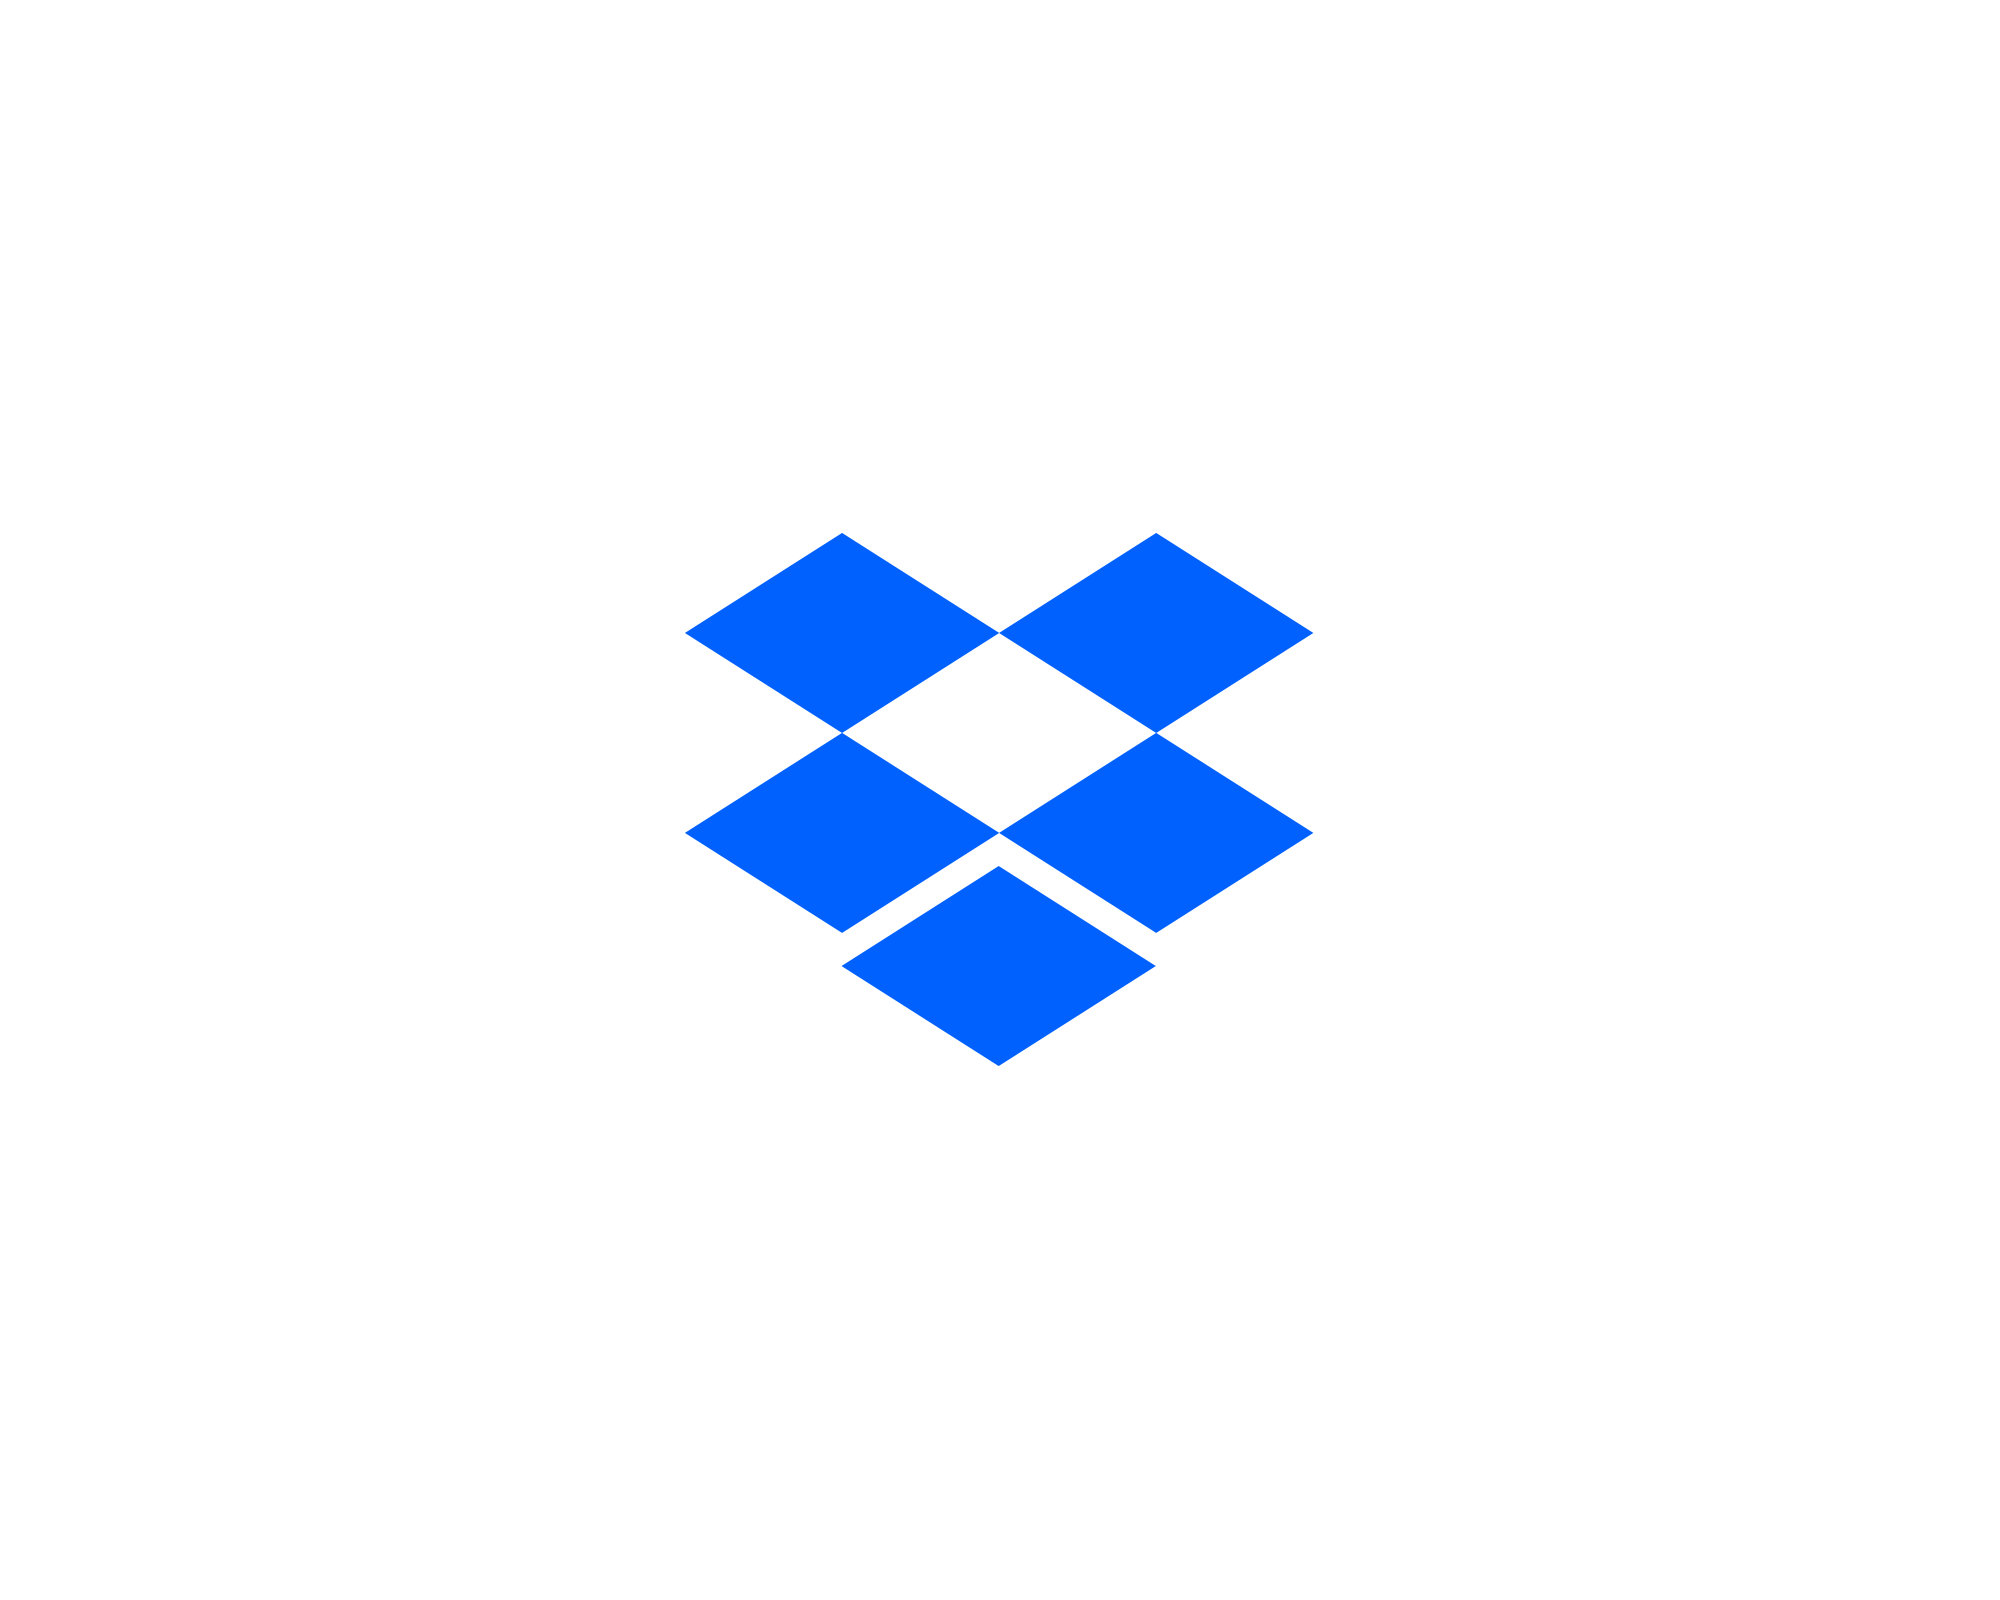
\includegraphics[scale=0.19]{logo.png}
 
%----------------------------------------------------------------------------------------
%	AUTHOR SECTION
%----------------------------------------------------------------------------------------
\begin{flushleft} \large
\emph{Autores:}\\
Antonio Gámiz Delgado \\
Samuel Medina Gutiérrez \\
Laura Sánchez Parra
\end{flushleft}

% If you don't want a supervisor, uncomment the two lines below and remove the section above
%\Large \emph{Author:}\\
%John \textsc{Smith}\\[3cm] % Your name


%----------------------------------------------------------------------------------------
%	LOGO SECTION
%----------------------------------------------------------------------------------------


 
%----------------------------------------------------------------------------------------

\vfill % Fill the rest of the page with whitespace

\end{titlepage}

\tableofcontents
\newpage

\section{Introducción}

Antes de hablar de Dropbox, vamos a comentar brevemente qué es el almacenanmiento en la nube y algunas formas de implementarlo:

Cloud-Storage es un modelo de servicio en el cual los datos son mantenidos, distribuidos, administrados y puestos a la disposición de los usuarios en una red (normalmente Internet). Los usuarios normalmente pagan por este servicio según su consumo, mensualmente, es decir, si quieres tener 5GB de almacenamiento en la nube, deberás pagar esos 5GB cada mes. 
Aunque el coste por cada GigaByte ha descendido enormemente, los proveedores de cloud storage han añadido más gastos “operativos” que puede hacer esta tecnología un poco más cara. Entre, los que por ejemplo, se encuentra la seguridad, que está siempre presente y en constante mejora ya que es una de las principales preocupaciones de los usuarios.

Este sistema presenta varias ventajas, como la facilidad de acceso a los datos desde cualquier punto con conexión a Internet, desde muchos tipos de dispositivos, la facilidad de recuperación de datos y el ahorro de los costes que conlleva comprar y mantener los propios sistemas de almacenamiento.

\section{Principales Sistemas de Almacenamiento.}

Un sistema de almacenamiento consiste en habilitar uno o varios discos duros de una red local (que a su vez puede estar conectada a Internet) de manera que los datos que allí se almacenen permanezcan accesibles a todos los dispositivos que deseen utilizarlos. De esta forma el usuario dispone de un almacenamiento común con el resto de usuarios.
La cuestión se complica cuando hay que definir la forma en que los distintos tipos de almacenamiento de datos gestionan esa conexión a tu red local.

\subsection{NAS - Network Attached Storage.}

Este sistema incorpora su propio sistema de conexión y recepción de petición de acceso a los datos, eliminando a los servidores de la ecuación. Los sistemas de almacenamiento NAS se conectan directamente al router (en local, LAN) mediante TCP/IP.

\subsection{SAN - Storage Area Network.}


Como un NAS, SAN traspasa la responsabilidad del almacenamiento de los datos de servidores y ordenadores a dispositivos de almacenamiento dedicados. Pero a diferencia de NAS, que es un dispositivo independiente, un SAN es una red de dispositivos de almacenamientos interconectados. Ambos son accedidos a través de la red local a la que están conectados.

Este tipo de sistema usa dos protocolos:
\begin{itemize}
\item Protocolo de canal de fibra (FCP): es la interfaz del protocolo SCSI (Small Computer System Interface) usando conexión de fibra óptica por debajo. Protocolo de alta velocidad que soporta la mayoría de canales y redes, ya que provee un estándar para el almacenamiento y la transferencia de datos.
\item Interfaz SCSI (iSCSI): protocolo que usa TCP/IP para la transferencia de datos. A diferencia del canal de fibra, solamente requiere Ethernet (o cualquier otra red compatible con TCP/IP) para funcionar. Esto permite soluciones menos costosas.
\end{itemize}

Dado que Dropbox es una empresa privada, nadie sabe exactamente cómo implementan su servicio de almacenamiento, pero se cree que usan mayormente SAN.

\section{Dropbox}

\subsection{¿Qué es Dropbox?}
Dropbox se define a si mismo como una CDN (Content Delivery Network), es decir, un conjunto de servidores que contienen copias de una misma serie de contenidos (imágenes, vídeos, documentos, etc) y que están ubicados en puntos diversos de una red para poder servir sus contenidos de manera más eficiente. Normalmente usan protocolos TCP/IP y TLS que reducen la latencia.
\subsection{Edge Network}
Para facilitar al usuario una mejor experiencia, se emplean protocolos TCP/IP y TLS más cercanos a los usuarios, ya que reducen la latencia, es decir, los retardos. Dropbox está formado por una serie de PoPs (Points of Presence) situados estratégicamente alrededor del mundo para reducir los tiempos de retardo.

Por lo que, la Edge Network de Dropbox es, el conjunto de PoPs que permiten reducir los tiempos de latencia.

\subsection{GSLB - Global Server Load Balancing}

¿Cómo distribuye Dropbox los usuarios entre los Pops? Utiliza GSLB, normalmente GSLB envía cada usuario al Pop más cercano, a no ser que el Pop este inhabilitado.

\subsubsection{BGP anycast}
Anycast es el método más fácil de loadbalancing. Usa el protocolo de routing del núcleo de Internet, BGP (Border Gateway Protocol - protocolo meidente el cuál se intercambia información de encaminamiento entre sistemas autónomos). Para empezar a usar anycast es suficiente con empezar a "publicar" la misma subred desde todos los PoPs e Internet entregerá cada paquete al PoP "óptimo" automáticamente. Aunque parece ser un muy buen método, tiene varias desventajas, como el limitado control que se tiene sobre el tráfico y es difícil mover tráfico implícitamente de un PoP a otro.

BGP anycast en Dropbox: debido a sus desventajas, sólo se usa para los dominos APEX, como dropbox.com (sin www) y como "último recurso" en caso de un ataque DDoS.

\subsubsection{GeoDNS}
En este método cada PoP tiene su propio y único espacio de direcciones IP y DNS es el responsable de asignar a IP diferente a cada usuario basado en su localización geográfica. Esto nos da más control sobre la dirección del tráfico, además, la configuración es más fácil y la solución de problemas es más simple.

GeoDNS en Dropbox: En este momento, están trabajando con el enrutamiento basado en LatLong (coordenadas geográficas), que es relativamente complejo.

\subsubsection{Hybrid unicast/anycast GSLB}

Combinación de las dos anteriores, que permite beneficiarse de las ventajas de los dos métodos.

\subsubsection{Real User Metrics}
Los métodos anteriores tienen un problema: ninguno de ellos usa datos de performance (actuación) percibido por los usuarios, sino que dependen en aproximaciones. Para arreglar eso, RUM usa datos de de las performances de los clientes de escritorio.

RUM en Dropbox: todavía es un proyecto en evolución que todavía no está implementado para el público general, pero se están realizando experimentos y recogiendo datos de los métodos anteriores para poder llegar a usar hasta 25-30 PoPs.

\subsection{Backbone Network}

Junto con la edge network, Dropbox ha creado una backbone network que permite la interconexión entre los data centers de Norte América, pero no sólo entre ellos, sino también con los nodos edge alrededor del mundo. ¿Por qué fue necesario crear tanto una edge network como una backbone network? Debido al número de usuarios  y la cantidad de datos que almacena cada uno de ellos y sobre todo al masivo crecimiento de los mismos, que hacía cada vez menos eficiente el almacenamiento en Dropbox. 

\subsection{Tipos de routers}
La red troncal de Dropbox consta de enrutadores con tres funciones distintas:
\begin{itemize}
\item Enrutadores del centro de datos (DR): con una función principal de conectar el centro de datos a la red troncal.
\item Enrutadores de red troncal (BB): que actúan como un punto de terminación para circuitos de larga distancia y también como dispositivos de agregación para DR en regiones donde tenemos centros de datos.
\item Peering Routers (PR): con una función principal de conectar Dropbox a pares BGP externos para proporcionar conectividad a Internet
\item Data Centers (DC): para conectar los data centers.
\end{itemize}

\subsection{Arquitectura de 2 niveles}

La red de Dropbox tiene dos tipos de tráfico: "tráfico de usuario" el cuál fluye entre Dropbox e Internet, y "tráfico del data center", el cuál fluye entre los data centers de Dropbox.

En la nueva arquitectura, existen dos dominios de red para manejar cada tipo de tráfico de forma independiente. El nivel DC lleva el tráfico del centro de datos, mientras que el nivel DR se usa para transportar el tráfico de usuarios, principalmente desde Dropbox a Internet. Cada nivel tiene su propia malla BGP, pero se conectan al mismo conjunto de enrutadores de red troncal (BB), que comparten la misma red de transporte físico.

El tráfico entre data centers es aproximadamente el doble del tráfico de usuarios y ambos tienen características diferentes. El tráfico del centro de datos consiste en servicios internos que se comunican entre sí o que copian datos de un centro de datos a otro. El tráfico de usuarios siempre se está transportando desde los DR a un punto de presencia, y se trata como tráfico premium. El despegue del tráfico interno de Dropbox a su propio nivel ha permitido una clara separación entre los dos tipos de tráfico, lo que ayuda a crear perfiles de tráfico y topologías de red que son únicas para cada tipo de tráfico.

\section{Dropbox LAN Sync}

Para terminar, vamos a hablar de una de las nuevas funciones de Dropbox, Dropbox LAN Sync:

Dropbox LAN Sync es una función que le permite descargar archivos de otras computadoras en su red, ahorrando tiempo y ancho de banda en comparación con descargarlos desde los servidores de Dropbox.
En vez de almacenar los archivos en los servidores de Dropbox, cualquier ordenador conectado a la misma red, podrá acceder a los demás  y descargar el archivo directamente desde allí sin tener que acceder a la nube.
Para comprender cómo funciona, primero debemos hablar de abstracciones que usa DropBox: Bloques y nameSpaces. Los archivos en DropBox están separados en bloques de 4MB direccionados por funciones HASH. Por tanto un archivo puede ser descrito por una lista de “Hashes”.

Los Espacios de nombre pueden ser pensados como directorios con permisos específicos. Cada cuenta tiene un espacio de nombre que representa su cuenta personal  y todos los archivos que contiene. 
En conclusión,  la petición de descargas de archivos puede pensarse como una serie de peticiones de pares (espacio de nombres, Hashes) para indicar el/los bloques específicos. Sin LAN Sync estas peticiones se meterían en una cola  y enviadas al servidor de bloques que devuelve un bloque de datos y por tanto no es necesario que la tubería de descarga conozca cosas como el nombre del archivo.

Esto también significa que LAN Sync  solo sincroniza los datos reales de los archivos  y no los metadatos. Asegurando que todos los metadatos recibidos provienen de los servidores de DropBox podemos tener la certeza de que todos están siempre en un estado consistente. Con el LAN Sync intentamos descargar los bloques directamente del peer de la conexión, accediendo si no es posible al servidor de bloques.

Esta tecnología tiene tres componentes principales:
\begin{itemize}
\item El “Discovery engine” que trata de encontrar máquinas que estén conectadas en la red que se puedan sincronizar. Para hacer esto cada máquina envía y escucha periódicamente de paquetes UDP sobre el puerto 17500. Estos paquetes contienen información sobre el protocolo usado, el espacio de nombres soportado…
\item Protocolo:  la transferencia del bloque se hace mediante HTTPS.
\item Servidor/Cliente: el servidor maneja peticiones de los clientes conectados en el servidor, proveyendo los bloques de datos solicitados. Los clientes solo son responsables de realizar las peticiones.  
\end{itemize}

\end{document}